%%%%%%%%%%%%%%%%%%%%%%%%%%%%% Define Article %%%%%%%%%%%%%%%%%%%%%%%%%%%%%%%%%%
\documentclass{article}
%%%%%%%%%%%%%%%%%%%%%%%%%%%%%%%%%%%%%%%%%%%%%%%%%%%%%%%%%%%%%%%%%%%%%%%%%%%%%%%

%%%%%%%%%%%%%%%%%%%%%%%%%%%%% Using Packages %%%%%%%%%%%%%%%%%%%%%%%%%%%%%%%%%%
\usepackage{geometry}
\usepackage{graphicx}
\usepackage{caption}
\usepackage{subcaption}
\usepackage{amssymb}
\usepackage{amsmath}
\usepackage{amsthm}
\usepackage{empheq}
\usepackage{mdframed}
\usepackage{booktabs}
\usepackage{lipsum}
\usepackage{graphicx}
\usepackage{color}
\usepackage{psfrag}
\usepackage{pgfplots}
\usepackage{bm}
\usepackage{float}
\usepackage{physics}
\usepackage{hyperref}
\usepackage{xcolor}
\usepackage{titlesec}
\usepackage{algorithmic}
\hypersetup{
	colorlinks=true,
	linkcolor=blue,
	filecolor=magenta,
	urlcolor=cyan
}
\usepackage{animate}
\usepackage{svg}
% Quantum physics inner product
\newcommand{\innerp}[2]{\left\langle #1 \vert #2 \right\rangle}
\newcommand{\convolution}[2]{(#1 \star #2)}

%%%  \begin{figure}[htp]
%%%  	\centering
%%%  	\includegraphics[width=0.25\textwidth]{/path/to/image}
%%%  	\caption{}\label{fig:}
%%%  \end{figure}

% to write multiple lines of equations

%%  \begin{align*}
%%  \begin{split}
%%  	\ket{\phi} + \ket{\psi} &= \ket{\phi + \psi} \\
%%  	a \ket{\psi} &= \ket{a \psi}
%%  \end{split}
%%  \end{align*}

\newcommand{\e}[1]{\times 10^{#1}}

\usepackage{listings}
\lstset{showstringspaces=false} % pretty embeded code in LaTeX
%%%%%%%%%%%%%%%%%%%%%%%%%%%%%%%%%%%%%%%%%%%%%%%%%%%%%%%%%%%%%%%%%%%%%%%%%%%%%%%

% Other Settings

%%%%%%%%%%%%%%%%%%%%%%%%%% Page Setting %%%%%%%%%%%%%%%%%%%%%%%%%%%%%%%%%%%%%%%
\geometry{a4paper}

%%%%%%%%%%%%%%%%%%%%%%%%%% Define some useful colors %%%%%%%%%%%%%%%%%%%%%%%%%%
\definecolor{ocre}{RGB}{243,102,25}
\definecolor{mygray}{RGB}{243,243,244}
\definecolor{deepGreen}{RGB}{26,111,0}
\definecolor{shallowGreen}{RGB}{235,255,255}
\definecolor{deepBlue}{RGB}{61,124,222}
\definecolor{shallowBlue}{RGB}{235,249,255}
%%%%%%%%%%%%%%%%%%%%%%%%%%%%%%%%%%%%%%%%%%%%%%%%%%%%%%%%%%%%%%%%%%%%%%%%%%%%%%%

%%%%%%%%%%%%%%%%%%%%%%%%%% Define an orangebox command %%%%%%%%%%%%%%%%%%%%%%%%
\newcommand\orangebox[1]{\fcolorbox{ocre}{mygray}{\hspace{1em}#1\hspace{1em}}}
%%%%%%%%%%%%%%%%%%%%%%%%%%%%%%%%%%%%%%%%%%%%%%%%%%%%%%%%%%%%%%%%%%%%%%%%%%%%%%%

%%%%%%%%%%%%%%%%%%%%%%%%%%%% English Environments %%%%%%%%%%%%%%%%%%%%%%%%%%%%%
\newtheoremstyle{mytheoremstyle}{3pt}{3pt}{\normalfont}{0cm}{\rmfamily\bfseries}{}{1em}{{\color{black}\thmname{#1}~\thmnumber{#2}}\thmnote{\,--\,#3}}
\newtheoremstyle{myproblemstyle}{3pt}{3pt}{\normalfont}{0cm}{\rmfamily\bfseries}{}{1em}{{\color{black}\thmname{#1}~\thmnumber{#2}}\thmnote{\,--\,#3}}
\theoremstyle{mytheoremstyle}
\newmdtheoremenv[linewidth=1pt,backgroundcolor=shallowGreen,linecolor=deepGreen,leftmargin=0pt,innerleftmargin=20pt,innerrightmargin=20pt,]{theorem}{Theorem}[section]
\theoremstyle{mytheoremstyle}
\newmdtheoremenv[linewidth=1pt,backgroundcolor=shallowBlue,linecolor=deepBlue,leftmargin=0pt,innerleftmargin=20pt,innerrightmargin=20pt,]{definition}{Definition}[section]
\theoremstyle{myproblemstyle}
\newmdtheoremenv[linecolor=black,leftmargin=0pt,innerleftmargin=10pt,innerrightmargin=10pt,]{problem}{Problem}[section]
%%%%%%%%%%%%%%%%%%%%%%%%%%%%%%%%%%%%%%%%%%%%%%%%%%%%%%%%%%%%%%%%%%%%%%%%%%%%%%%

%%%%%%%%%%%%%%%%%%%%%%%%%%%%%%% Plotting Settings %%%%%%%%%%%%%%%%%%%%%%%%%%%%%
\usepgfplotslibrary{colorbrewer}
\pgfplotsset{width=8cm,compat=1.9}
%%%%%%%%%%%%%%%%%%%%%%%%%%%%%%%%%%%%%%%%%%%%%%%%%%%%%%%%%%%%%%%%%%%%%%%%%%%%%%%

%% Centering section titles
\titleformat{\section}[block]{\Large\bfseries\filcenter}{}{1em}{}

%% norm
%%\newcommand\norm[1]{\lVert #1 \rVert}


\title{Machine Learning}
\author{Aheer Srabon}

\begin{document}
\maketitle

\section*{Learning}

\subsection*{K-Means Algorithm}
\noindent Input to the algorithm are,
\begin{itemize}
\itemsep0em
	\item K (number of clusters)
	\item Training set $ {x^{(1), ..., x^{(m)}}} $
\end{itemize}

\noindent At first, K points are randomly initialized. In the \emph{Cluster assignment} step, each
of $ x^{(i)} $ is assigned a cluster number (1 to K) depending on how close the point $ x^{(i)} $
to a specific cluster centroid. In the \emph{Move centroid} step, mean of the points which are
assigned to the a particular cluster number is calculated and assigned to the cluster centroid of that
cluster centroid. Following is the algorithm,

\noindent Randomly initialize $ K $ cluster centroids $ \mu_1, \mu_2, ... , \mu_K \in \mathbb{R}^n $.

\begin{algorithmic}
	Repeat {
		
	}
\end{algorithmic}

\subsection*{Dimensionality Reduction using PCA}
\noindent \textbf{Data Compression: } Reduce data from 2D to 1D,
or reduce data from 3D to 2D. Reduces the number of features
that the data has.
\begin{itemize}
\itemsep0em
	\item Saves storage space
	\item Makes the learning algorithm run faster (important)
\end{itemize}
\vspace{0.5em}
\noindent A dataset which has a huge number of features make the
learning algorithm run very slow. That is why, PCA is applied to
keep the data while discarding less important data of the data.

\vspace{0.5cm}

\noindent \textbf{Data Visualization: } It may be often insightful
to see the data visually. But higher dimensional data can't be
seen by human beings. That is why, PCA is applied to better observe
the data visually.

\subsection*{Principal Component Analysis (PCA)}

\noindent \textbf{Problem formulation: } Find $ k $ vectors 
$ u^{(1)}, u^{(2)}, ... , u^{(k)} $ onto which to project the data, so
as to  minimize the \textbf{projection error}.

\vspace{0.3cm}

\noindent Informally, project the data onto the linear subspace,
spanned by the $ k $ vectors $ u^{(1)}, u^{(2)}, ... , u^{(k)} $.

\vspace{0.5cm}

\begin{figure}[htp]
	\centering
	\begin{subfigure}{.5\textwidth}
		\centering
		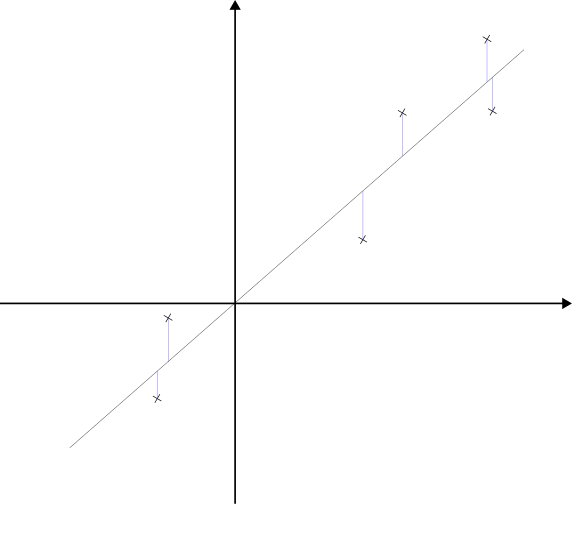
\includegraphics[width=.85\linewidth]{./assets/linear_regression.png}
		\caption{Linear regression (minimize squared distances)}
	\end{subfigure}%
	\begin{subfigure}{.5\textwidth}
		\centering
		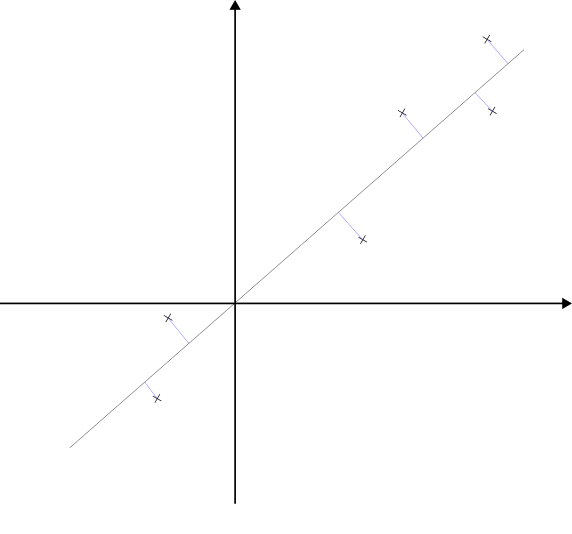
\includegraphics[width=.85\linewidth]{./assets/pca.png}
		\caption{PCA (minimize squared distances)}
	\end{subfigure}
	\caption{Linear regression vs PCA}
\end{figure}

\vspace{0.5cm}

\noindent Let the training data be, $ x^{(1)}, x^{(2)}, ... , x^{(m)} $

\noindent \textbf{Data preprocessing: }
\vspace{0.3cm}
\noindent\emph{Mean normalization: } 

\noindent Calculate mean of $ i $th feature of the data set,
\begin{equation}
	\mu^{(i)} = \frac{1}{m} \sum_{j=1}^{m} x_j^{(i)}
\end{equation}

\begin{equation}
	x^{(i)} \leftarrow x^{(i)} - \mu^{(i)} 
\end{equation}


\noindent\emph{Feature scaling: }
\begin{equation}
	x^{(i)} \leftarrow \frac{x^{(i)} - \mu^{(i)}}{S^{(i)}}
\end{equation}

\noindent Here, $ S^{(i)} $ is a measure of variation in the data of $ i $
th feature. Mostly, it is set to be the standard deviation of the data.

\vspace{0.5cm}

\noindent \textbf{Principal component analysis (Algorithm): }
\noindent The data is stored in a matrix $ X \in \mathbb{R}^{m \times n} $, where
each row represents a certain point in the data space (a reading), and each column
represents one feature. So there are $ m $ readings and $ n $ features.

\vspace{0.3cm}

\noindent \textbf{Step 1:} Compute the covariance matrix,
\begin{equation}
	\Sigma = \frac{1}{m} \sum_{i=1}^{n} (x^{(i)}) (x^{(i)})^T; 
	\hspace{1cm} (\Sigma \in \mathbb{R}^{n \times n})
\end{equation}

\vspace{0.25cm}

\noindent \emph{Matlab specific implemementation:} $ Sigma = \frac{1}{m} (X' X) $

\vspace{0.5cm}

\noindent \textbf{Step 2:} Find the eigenvectors of the covariance matrix,
\begin{center}
	[U, S, V] = svd(Sigma)
\end{center}

\noindent Here, $ U $ is the matrix whose columns are the eigenvectors of the matrix $ \Sigma $.
$ U \in \mathbb{R}^{(n \times n)} $

\vspace{0.5cm}

\noindent \textbf{Step 3:} Take the first $ k $ columns of the eigenvector matrix $ (U) $ and call
it $ U_{reduced} $. 

\noindent $ U_{reduced} \in \mathbb{R}^{(n \times k)} $

\vspace{0.25cm}

\noindent \emph{Matlab specific implemementation:} Ureduce = U(:, 1:k)

\vspace{0.5cm}

\noindent \textbf{Step 4:} Multiply each example $ x^{(i)} $ with $ u_{reduced} $ to get the reduced
version of the example. For a column vector example $ x \in \mathbb{R}^{(n \times 1)} $ which has 
$ n $ entries as values of its $ n $ features (notice that the bias is not included), its reduced
form can be found with the following equation,

\begin{equation}
	z = U_{reduced}' x
\end{equation}

\noindent Originally, $ x \in \mathbb{R}^{(n \times 1)} $. The reduced form of $ x $ is
$ z \in \mathbb{R}^{(k \times 1)} $.

\vspace{0.25cm}

\noindent \emph{Matlab specific implemementation:} $ Z = X * U_{reduced} $.
Here, $ X \in \mathbb{R}^{(m \times n)} $, $ U_{reduced} \in \mathbb{R}^{(n \times k)} $. So,
$ Z \in \mathbb{R}^{(m \times k)} $. The number of columns got reduced from $ n $ to $ k $, which
indicates reduction in dimensions of the data.

\noindent \textbf{Reconstruction from compressed representation: }
\noindent To reduce one training example $ x $ from $ n $ dimension to $ k $ dimensions,

\begin{equation}
	z = U_{reduce}^T x
\end{equation}

\noindent Now, given the compressed form $ z $, original $ n $ dimensional vector $ x $ can be
approximated by,
\begin{equation}
	x_{approx} = U_{reduce} z
\end{equation}

\noindent \textbf{Chossing the number of principal components: }
\noindent PCA tries to minimize the \emph{average squared projection error},
\begin{equation}
	\frac{1}{m} \sum_{i=1}^{m} \norm{x^{(i)} - x_{approx}^{(i)}}^2
\end{equation}

\noindent Total variation in the data is defined as,
\begin{equation}
	\frac{1}{m} \sum_{i=1}^{m} \norm{x^{(i)}}^2
\end{equation}

\noindent Choose $ k $ to be smallest values such that,
\begin{equation}
	\frac{\frac{1}{m} \sum_{i=1}^{m} \norm{x^{(i)} - x_{approx}^{(i)}}^2}
	{\frac{1}{m} \sum_{i=1}^{m} \norm{x^{(i)}}^2} \leq 0.01
\end{equation}
\noindent \orangebox{99\% of the variance is retained}

\vspace{0.5cm}

\noindent \textbf{Step 1:} Try PCA with $ k = 1 $

\noindent \textbf{Step 2:} Compute $ U_{reduce}, z^{(1)}, ..., z^{(m)}, x_{approx}^{(1)}, ..., x_{approx}^{(m)} $

\noindent \textbf{Step 3:} Check if,
\begin{equation}
	\frac{\frac{1}{m} \sum_{i=1}^{m} \norm{x^{(i)} - x_{approx}^{(i)}}^2}
	{\frac{1}{m} \sum_{i=1}^{m} \norm{x^{(i)}}^2} \leq 0.01
\end{equation}

\noindent If it is, stop. Otherwise, repeat from the start with $ k \leftarrow k + 1 $

\vspace{0.5cm}

\noindent But this procedure is not efficient. While computing $ U, S, V $ using \emph{svd}, we only used
the matrix $ U $, containing the eigenvectors. But, $ S $ can be used when choosing the number of principal
components. $ S \in \mathbb{R}^{(n \times n)} $ is a diagonal matrix with entries $ S_{11} ,..., S{nn} $.

\begin{equation}
	\frac{\sum_{i=1}^{k} S_{ii}}{\sum_{i=1}^{n} S_{ii}} \geq 0.99
	\label{eq:12}
\end{equation}

\noindent So, apply \emph{svd} on $ \Sigma $ to find the matrix $ S $. Use this $ S $ matrix to choose $ k $
using equation \ref{eq:12}.

\vspace{0.5cm}

\pagebreak

\noindent A couple of points to note regarding PCA,

\begin{description}
	\item[DO: Speeding up the learning algorithm] \hfill \\
		$ (x^{(1)}, y^{(1)}), ..., (x^{(m)}, y^{(m)}) $ and $ x^{(i)} \in \mathbb{R}^{(100 \times 100)} $.
		Extract the inputs, $ x^{(1)}, ... , x^{(m)} \in \mathbb{R}^{(100 \times 100)} $.
		Apply PCA, $ z^{(1)}, ..., z^{(m)} \in \mathbb{R}^{(30 \times 30)} $.
		The new training set is now, $ (z^{(1)}, y^{(1)}), ..., (z^{(m)}, y^{(m)}) $.
		Feed this new training set into the learning algorithm $ h_\theta (z) \rightarrow y $. When a new
		training example is encountered, $ z = U_{reduce}^T x $ and $ h_\theta(z) \rightarrow y $.

		This mapping ($ x \rightarrow z) $ should only be \emph{defined} by running PCA on the training
		set, which is then applied to $ x_{cv} $ and $ x_{test} $.

	\item[Don't: Preventing overfitting] \hfill \\
		PCA should not be used to prevent overfitting. Because it reduces the dimension of the input
		data without considering the labels ($ y^{(i)} $). Instead, use regularization to prevent
		overfitting.

	\item[Don't: Design ML systems] \hfill \\
		PCA throws away information. At first, use original data in the learning algorithm. Only when
		the original data doesn't accomplish the desired objective, use PCA.

\end{description}

\end{document}
